\documentclass[]{emulateapj}
\usepackage{amsmath}
\begin{document}
\author{Draft}




\section{CO($J$ = 3 $\rightarrow$ 2) line emission}
%- ! Parameters and Errors:
%- ! MFIT%PAR[01]  
%- ! MFIT%PAR[02]  
%- ! MFIT%PAR[03]  
%- ! MFIT%PAR[04]  
%- channel [, ]
%- velocity range [,] km/s
%- Integrated line flux =
%- rms =

%We have detected unresolved CO($J$ = 3 $\rightarrow$ 2) line emission toward SMM J0939+8315 at peak flux
%of blah sigma  of $ \sigma$ = blah mJy beam$^{-1}$.

We detect unresolved CO($J$ = 3 $\rightarrow$ 2) line emission toward the background galaxies in RXJ1131-1231. 
We extract the spectrum and fit a single-component Gaussian as shown in Figure \ref{fig:CO32mom0}, 
yielding peak flux density of BLAH $\pm$ BLAH mJy, the FWHM of the Gaussian fit is BLAH $\pm$ BLAH km s$^{-1}$. 


%No significant continuum emission is detected from the line-free region down to a 1$\sigma$ limit of blah mJy. 


\section{CO($J$ = 2 $\rightarrow$ 1) line emission}
We detect dynamically resolved CO($J$ = 3 $\rightarrow$ 2) line emission toward the background galaxies in RXJ1131-1231. 

We construct the velocity-integrated (0th moment) map of the CO($J$ = 2 $\rightarrow$ 1) emission using the uv-continuum subtracted data, the velocity-integrated CO($J$ = 2 $\rightarrow$ 1) line flux is BLAH $\pm$ BLAH Jy km s$^{-1}$.

% upper limit on other lines 
% in the background source -- H2CO 

% in the foreground galaxy -- H2CO, HNC (J=2-1)
\begin{figure*}[tbph]
\centering
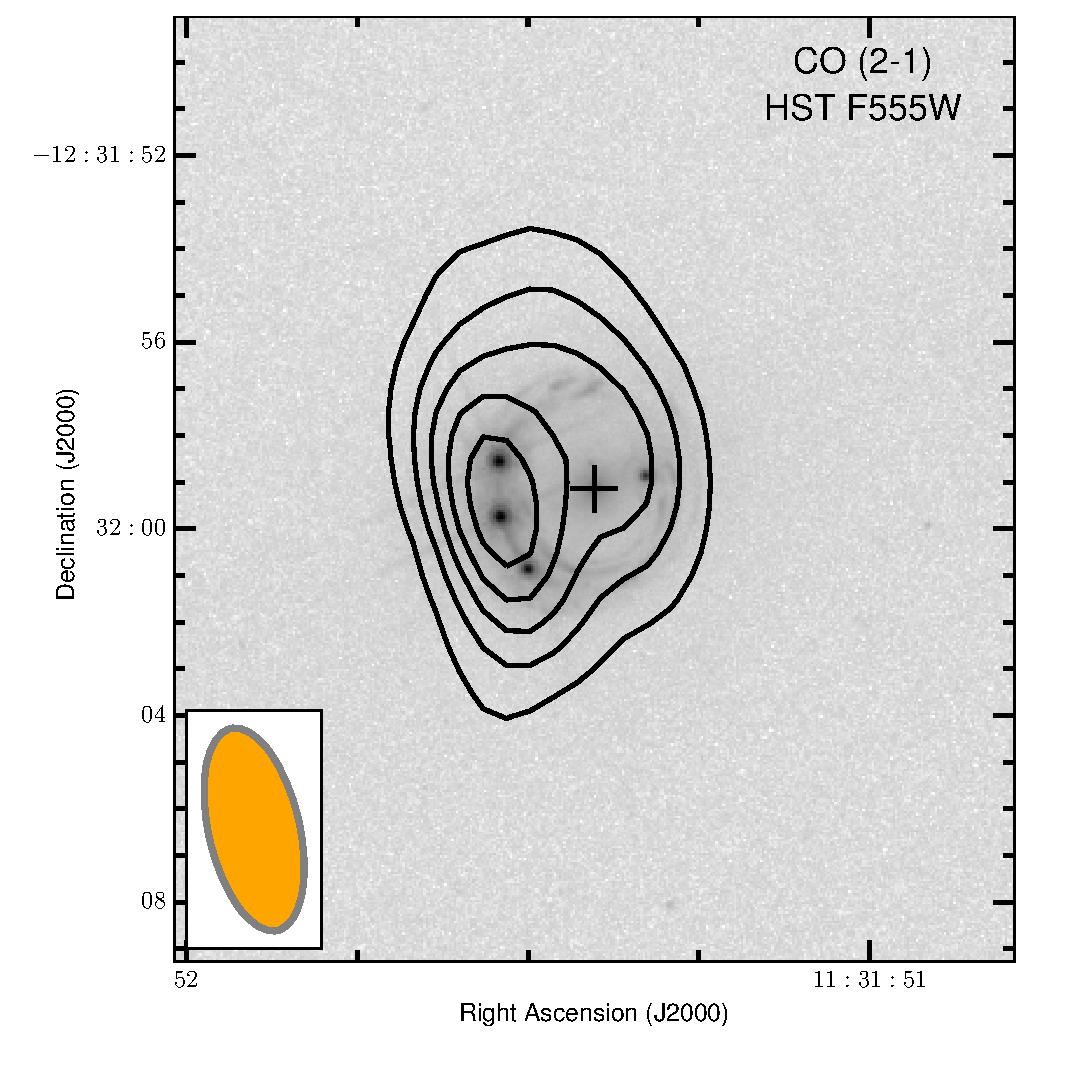
\includegraphics[width=0.35\textwidth]{../Figures/F555WCO21_mom0_single_invertedgray.eps}       % figures are in ../Figures/ for now, before we decided which ones will definitely go into paper
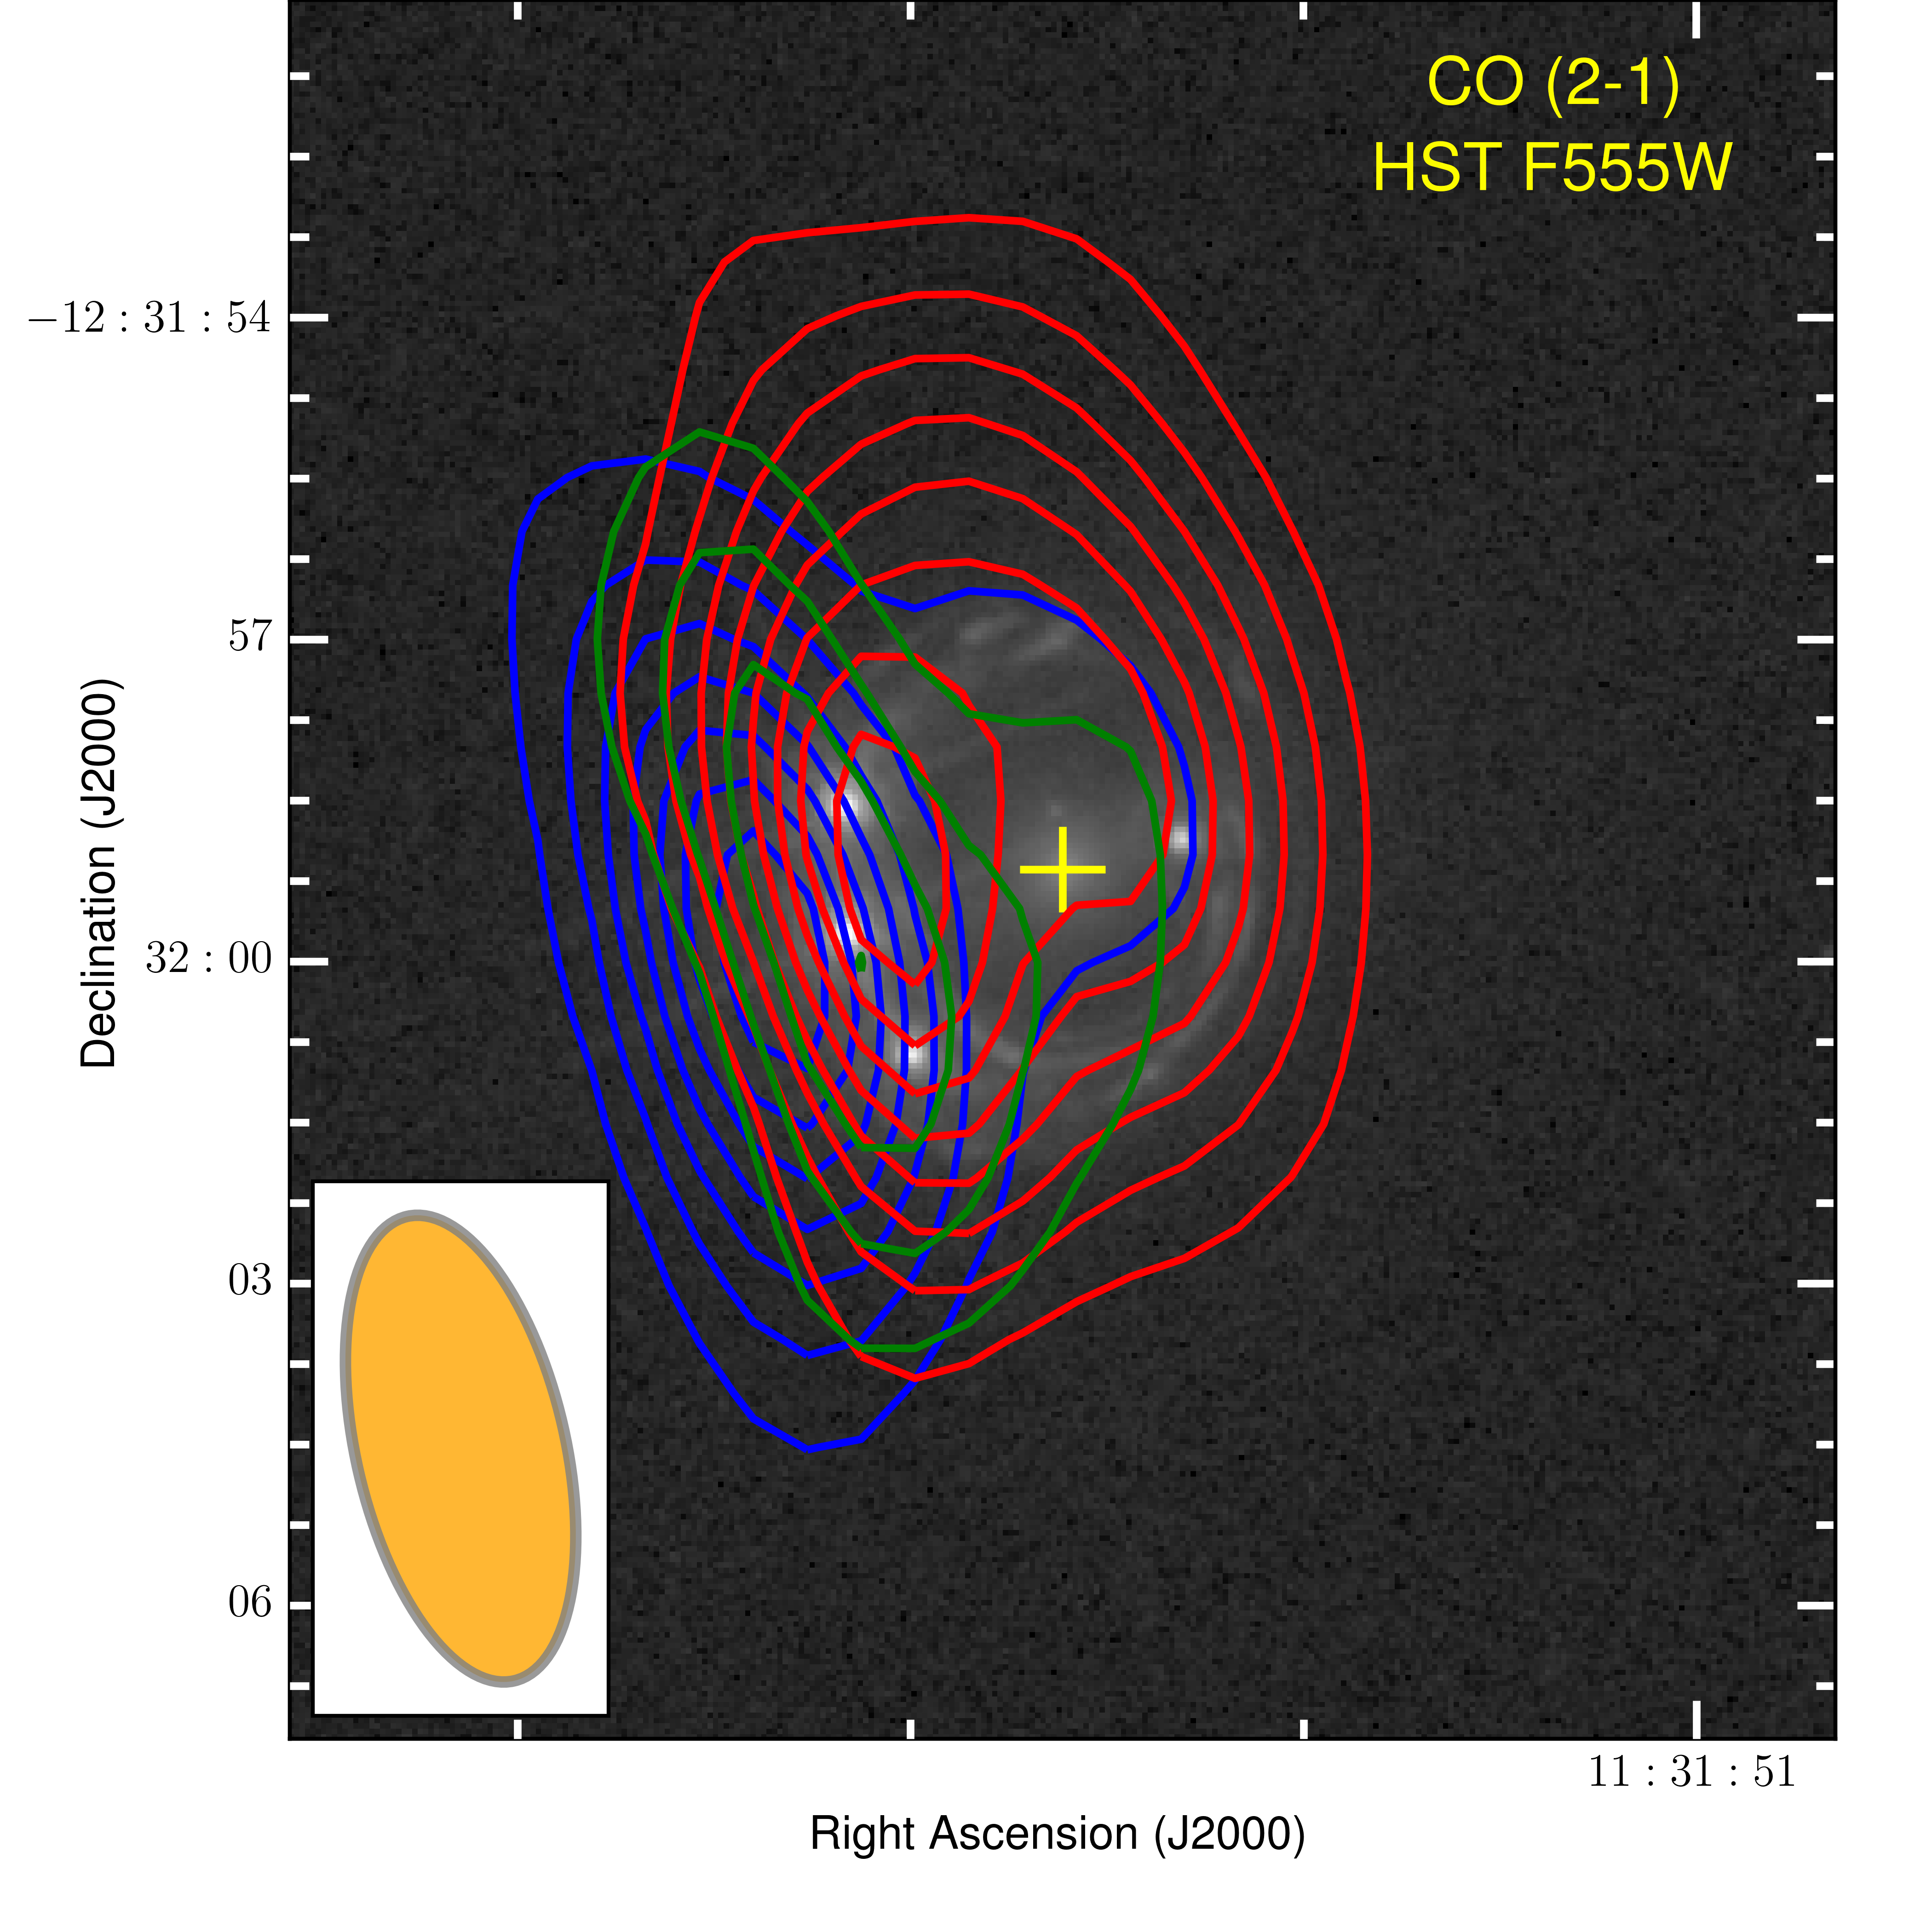
\includegraphics[width=0.35\textwidth]{../Figures/F555W_REDCentBLUE.png}
\includegraphics[width=0.55\textwidth]{../Figures/SpecCO21_twinx.eps}
\caption{
0th Moment map of CO(2-1) emission on HST F555W.
Spectrum. Velocity scale w.r.t z=0.655
 \label{fig:CO21mom0}}
\end{figure*}


\begin{figure}[tbph]
\centering
\includegraphics[width=0.5\textwidth]{../Figures/CO_highOmom_CLIP5sigma}       % figures are in ../Figures/ for now, before we decided which ones will definitely go into paper
\caption{
1st and 2nd order moments
 \label{fig:}}
\end{figure}




\begin{figure*}[tbph]
\centering
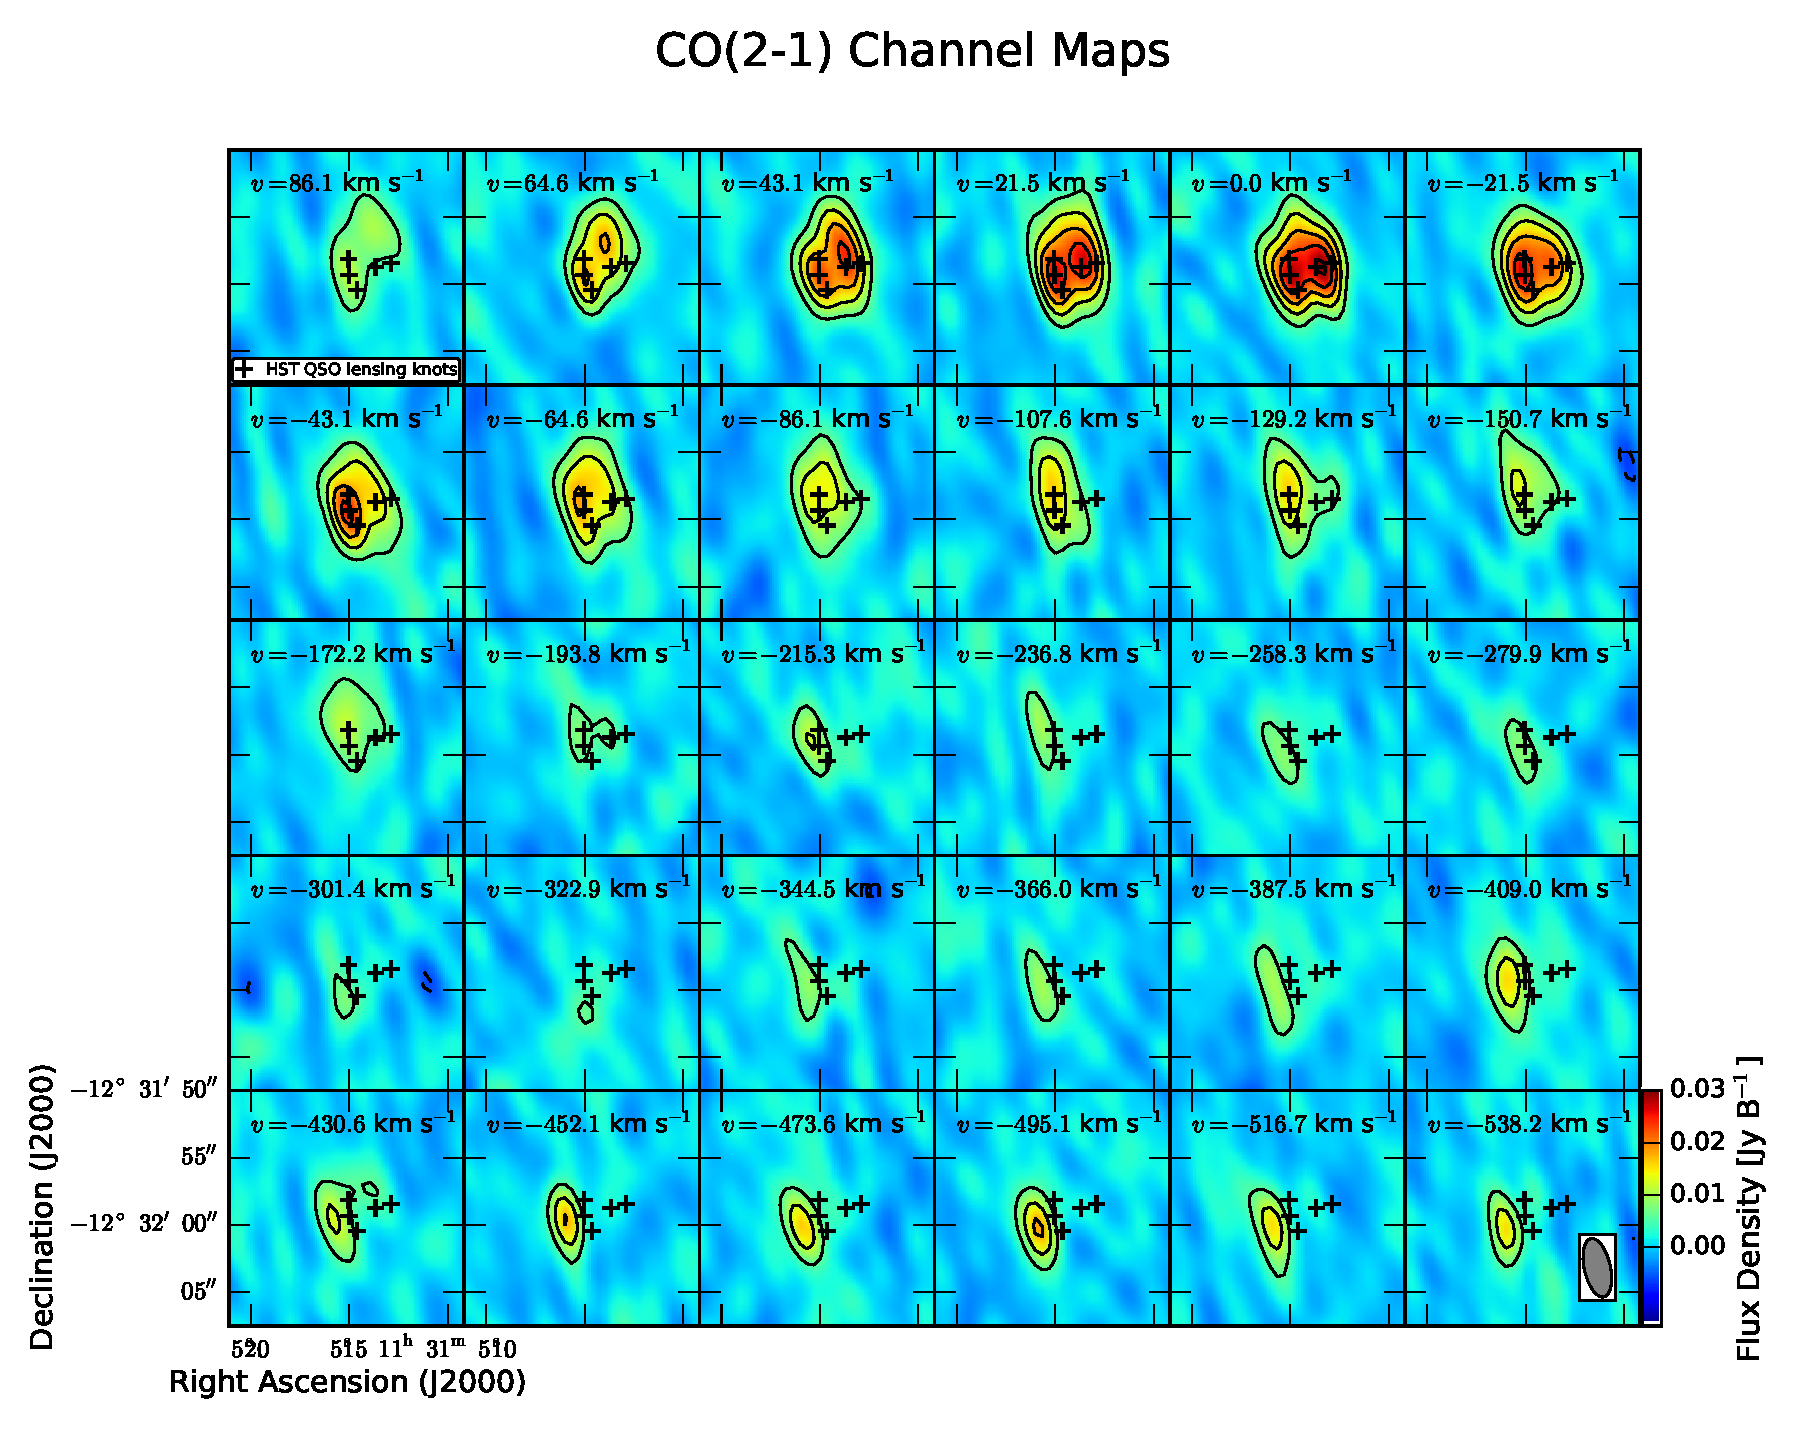
\includegraphics[width=\textwidth]{../Figures/co_channel_maps.eps}       % figures are in ../Figures/ for now, before we decided which ones will definitely go into paper
\caption{
Black crosses indicate the position of the lensed AGN (components ABCD) and the foreground lensing galaxy (component G) in the HST image.
 \label{fig:chanmap}}
\end{figure*}

\begin{figure*}[tbph]
\centering
\includegraphics[width=\textwidth]{../Figures/spatialSpec_offsetShifted.eps}       % figures are in ../Figures/ for now, before we decided which ones will definitely go into paper
\caption{ 
Spatial spectra, binned by 3 pixels in each direction (1\farcs5)
 \label{fig:spatialSpec}}
\end{figure*}

%
%\begin{figure*}[tbph]
%\centering
%\includegraphics[width=0.8\textwidth]{}       % figures are in ../Figures/ for now, before we decided which ones will definitely go into paper
%\includegraphics[width=0.65\textwidth]{}
%\caption{
% \label{fig:}}
%\end{figure*}

\section{Continuum}

%
%\begin{figure*}[tbph]
%\centering
%\includegraphics[width=0.80\textwidth]{}
%\caption{Left: Contours of the CARMA BLAH GHz continuum emission (red) in the foreground radio galaxy 3C220.3 overlaid on the image and contours of the VLA 6 GHz continuum emission (lime). The rms in the VLA 6 GHz continuum image is $\sigma$ = 0.0641 mJy beam$^{-1}$. The synthesized beam size is 0$\farcs$596 $\times$ 0$\farcs$229, at P.A. 75.79$\degr$. Lime contour levels start at $\pm$4$\times\sigma$ = x mJy beam$^{-1}$ and increment at steps of $\pm$2$\sigma$ for the VLA data; red contour levels start at $\pm$2$\sigma$, incrementing at steps of $\pm$1$\sigma$ = 0.24 mJy beam$^{-1}$.
%Right:
%Contour map of the 90.7 GHz continuum emission. The beam size is 16\farcs67$\pm
%$0\farcs69 $\times$ 7\farcs17$\pm$1\farcs60, at P.A. = -57.9$\degr$. The contour levels start at $\pm$2$\sigma$ and increment at steps of $\pm$1$\sigma$ =0.5 mJy beam$^{-1}$.\label{fig:cont}}
%\end{figure*}




%%%%%%%%%%%%%%%
\end{document}